\subsection{论文要回答的问题}

常规统计直觉认为样本越大推断越准。论文指出，个体超传播、不完全报告和共同环境扰动同时存在时，病例数与推断信息量之间的关系取决于估计目标。若目标是当期传播参数 $R_t$（论文称为目标 A），测量方差随期望报告规模 $m=\rho n$ 单调趋于零；若目标是跨期基础传播水平 $\bar R$（目标 B），单期估计留有一个不随规模下降的环境方差 $v_R$。论文据此把“病例规模在什么条件下不再主导推断误差”写成一个可计算的监测设计问题，核心量是规模项与环境项相等时的期望报告规模 $m_\times=A/v_R$。

\subsection{核心结论}

\begin{enumerate}
\item 命题 1 证明，给定上一代感染者数 $n$ 与当期 $R_t$，报告病例数 $C_t$ 严格服从负二项分布，$C_t/(\rho n)$ 是 $R_t$ 的最大似然估计，且在每个有限 $n$ 上精确达到 Cram\'er--Rao 下界，方差为 $R_t/(\rho n)+R_t^2/(kn)$，随规模单调趋于零。
\item 命题 2 用全方差公式把目标 B 的单期方差写成 $v_R+A/m$，其中 $A=\bar R+\rho(\bar R^2+v_R)/k$。环境项 $v_R$ 与规模无关，构成单期推断的方差下限。
\item 定义 1 给出交叉点 $m_\times=A/v_R$。在 $m=m_\times$ 处两项各占一半，规模翻倍带来的方差降幅为 $1/[2(1+m/m_\times)]$。以论文图 1 的参数（$\bar R=1.15$、$v_R=0.04$、$k=0.35$、$\rho=0.25$）计算，$A=2.1232$，$m_\times=53.08$，翻倍降幅在 $m=10$、$m_\times$、$200$ 处分别为 42.1\%、25.0\%、10.5\%。
\item 命题 3 比较两条扩大规模的路径：提高报告率 $\rho$ 只能消除漏报带来的抽样方差，扩大感染基数 $n$ 能让全部规模项同时衰减。
\item 命题 4 与推论 1 处理预算分配。在每期固定成本 $c_0$ 与单例成本 $c_1$ 下，最优单期规模为 $m^*=\sqrt{(c_0/c_1)m_\times}$，在 $c_0/c_1=10$ 与 $100$ 时分别为 23.0 与 72.9。环境扰动存在 AR(1) 相关时，有效期数近似 $T(1-r)/(1+r)$ 恒高估环境项，在 $T=26$、$r=0.8$ 时高估 20.5\%。
\item 命题 5 分解单步预测方差，命题 6 给出超临界增长的精确离散检验。离散检验的功效随 $n$ 呈锯齿状变化，在 $k=0.35$、$\delta=0.30$ 时功效首次达到 0.8 的样本量为 568，此后不再跌回 0.8 以下的稳定样本量为 581。
\item 实证部分使用全美 CDC NHSN 流感住院数据（16,218 个州周观测）。流行初期相对均方误差按 $a+b/D_t$ 递减，经验交叉点约 22.6 例/周，39\%--55\% 的误差份额落在与规模无关的截距上；达峰期常数均值偏移占总误差的 88.9\%。在 FluSight 集成预测和欧洲 11 国 COVID-19 数据中，规模项均为正，多模型集成把达峰期均值偏差占比压缩到 15.5\%。
\end{enumerate}

\subsection{逻辑链}

图~\ref{fig:logic} 给出全文的依赖关系。左列是两条模型假设，负二项分支传播与二项报告抽样共同给出命题 1 的单期精确分布。命题 1 在环境层取全方差得到命题 2，命题 2 的两项之比定义交叉点。交叉点再分别进入报告率与基数的比较（命题 3）、预算分配（命题 4 与推论 1）、预测分解（命题 5）和增长检验（命题 6）。右列是两类检验：命题 3 与命题 4 的规模关系由美国流感住院数据检验，命题 5 与命题 6 由更新过程仿真检验。虚线表示实证截距、斜率与理论参数之间的口径差，第~\ref{sec:empirical} 节与第~\ref{sec:checks} 节专门讨论这一反馈。

\begin{figure}[!tbp]
\centering
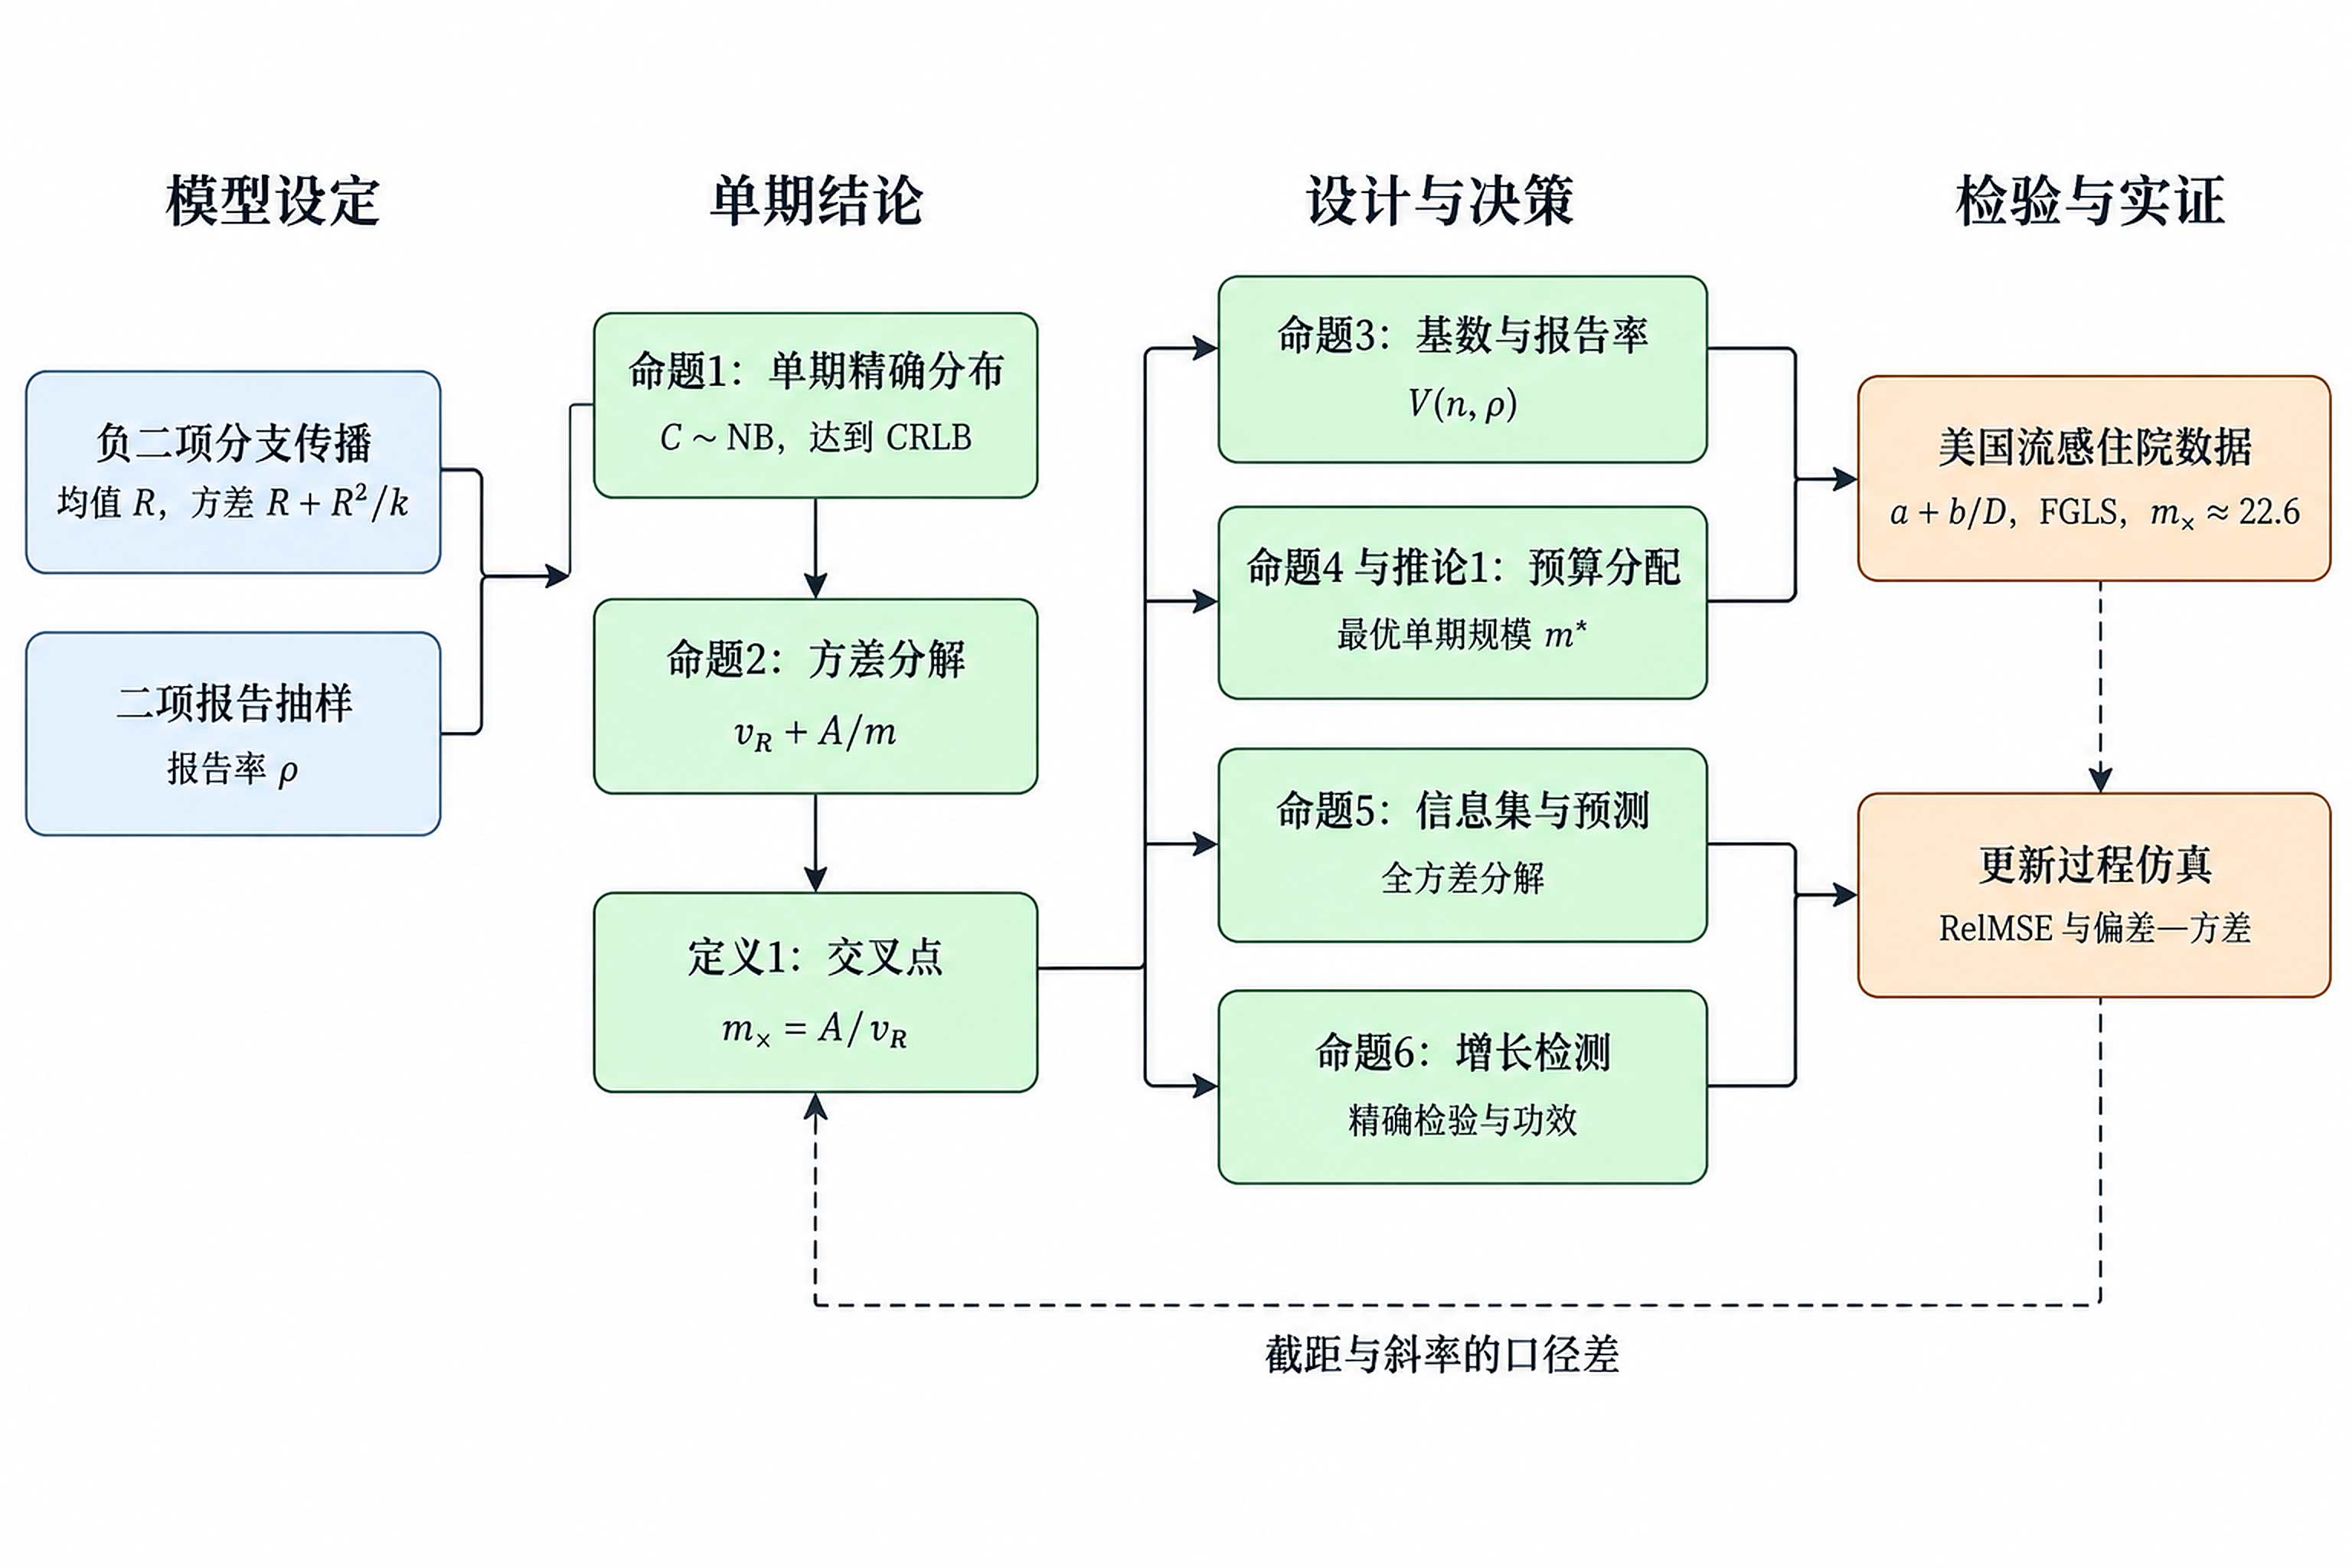
\includegraphics[width=0.95\linewidth]{figures/fig_logic_chain.png}
\caption{全文逻辑链。蓝色框是模型假设，绿色框是理论结论，橙色框是仿真与实证检验；实线箭头表示推导依赖，虚线表示实证截距与斜率和理论参数之间的口径差对交叉点定义的反馈。}
\label{fig:logic}
\end{figure}

\subsection{阅读建议}

第~\ref{sec:prereq} 节列出十项前置知识，前四项（负二项分布与概率生成函数、Fisher 信息与 Cram\'er--Rao 下界、全方差公式、AR(1) 有效样本量）是读懂第~\ref{sec:props} 节的必要条件。第~\ref{sec:symbols} 节与第~\ref{sec:model} 节可作为查阅表，推导中遇到陌生符号时回查。第~\ref{sec:props} 节建议按命题 1、命题 2、定义 1 的顺序在纸上逐步重推，这三步是答辩时最可能被要求现场推导的内容；命题 3 至命题 6 可在掌握前三步后按需阅读。第~\ref{sec:empirical} 节与第~\ref{sec:checks} 节对应答辩中关于实证口径的追问，第~\ref{sec:advice} 节给出修改方案与问答准备。附录~\ref{app:lemmas} 收录四个基础引理的完整证明，正文推导引用它们时不再重复。
